\documentclass[11pt,a4paper]{report}
\usepackage[utf8]{inputenc}
\usepackage{amsmath}
\usepackage{amsfonts}
\usepackage{amssymb}
\usepackage{graphicx}
\author{Jan Dziedzic}
\usepackage{fancyhdr}
\title{PycMan}
\fancypagestyle{}{%
\fancyhf{} % clear all header and footer fields
\fancyhead[RE,LO]{\chaptername \thechapter}
\renewcommand{\headrulewidth}{0pt}
\renewcommand{\footrulewidth}{0pt}}
\renewcommand{\chaptername}{Part}

\newenvironment{img}{
	\begin{center}
		\begin{figure}
			\begin{center}
			
}{
	\end{center}
		\end{figure}
			\end{center}
}

\begin{document}
	\maketitle
	\newpage
	\thispagestyle{empty}
	$$$$
	\newpage
	\thispagestyle{empty}
	\tableofcontents
	\chapter{Project Definition and Analysis}
		\newpage
		\section{Project Definition}
			As my project, I have decided to present a game written in Python, based around one of its modules - pygame. As I have not had as much time to prepare my project as my colleagues, I have decided that the concept of the game must be simple, yet allowing to demonstrate my programming and computational thinking skills. For this purpose I have decided to mimic the iconic PacMan game.
			For picture of the original game screen please refer to Figure \ref{oryg_pacman}
			
			\begin{img}
				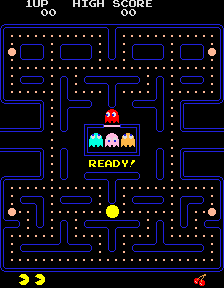
\includegraphics{images/1_1}\\
				\caption{Original Pac-Man screen. Source is Reference \ref{stronaopacmanie}.}
				\label{oryg_pacman}
			\end{img}
		
			Called PycMan (utilizing the fact that many of Python modules have a prefix 'py' in their name), the game itself strongly resembles the original, yet with some meaningful changes. Like in the original - player can move in four directions (left, right, up and down), collecting coins and avoiding ghosts.
			
			
			The game develops critical thinking skills and takes effect of human nature of taking risks and tackling unknown - with having more confidence when predicting ghost behavior, the player actually gets better when playing despite problems generally low complexity.
			
			Actually the game itself may be referred as to playing tag in a transparent maze. Such a play would be very hard for a human to enjoy as analyzing transparent walls while running and predicting opponent's next move is a far too complex problem for human cognition. That's why computational approach on this game is required - where player can see ghosts from above the board whilst ghost may exhibit algorithmically advanced behavior.
		\section{Stakeholders}
			Proposed end user group is really wide. As the game itself can be launched on virtually any device due to Python versatility, it may be used on a spectrum of devices with different controllers, from mobile phones and smart watches through PCs reaching as far as game console emulators mimicking the most authentic PacMan game experience. Such portability should satisfy most users.
			
			The game should grab attention of children - with small challenges that don't require complex thinking and rather promote manual skills and reflex; those who seek quick brainteaser whilst attempting to play with more focus on tactics of ghost avoidance and finally, old gamers who played original PacMan but now they might want to try more modern version with a different approach to critical game mechanisms.
		\section{Software Challenges}
			All software used to develop the game but is not necessarily required to run it:
			\begin{itemize}
				\item Python3
				\subitem Pillow module
				\subitem Pygame module
				\item Pycharm Professional
				\item GIMP - GNU Image Manipulation Program
				\item \LaTeX
				\item TeXstudio
			\end{itemize}
			
			The greatest advantage that convinced me to actually use Python for my game was its portability. As an interpretable programming language, the code of the game remains universal throughout different operating systems and processor architectures. My decision was also influenced by my previous experience with this language and my desire to actually get better around it.
			
			Also, whilst most of my experience was with Python2 I have decided that it's the right time to move on and actually start using Python3, which is reportedly faster and offers more functionality while providing greater stability.
			
			Still, Python does not offer the speed one may expect from a programming language suitable for complex games. Advanced non-optimal solutions need to be thought of and substituted with faster algorithms in order for the game to run smooth on machines lacking processing power.
			
			Pycharm by JetBrains was used as a Python IDE - it is a really convinient solution and comes with a lot of useful features. It was chosen due to my previous positive experience with it.
			
			GIMP was used to produce graphics resources of the game as well as levels - described later.
			
			\LaTeX and Texstudio were used to develop this document.
			
			All development was done on an Ubuntu-running computer, therefore	
			I must proudly admit that during the entire design process no non-free software was used. All software was either opensource, freeware or free for education.
			
		\section{The Interview}
			To assess interest and gain insight of the potential market for the game, I have interviewed my fellow schoolmate - Wojciech Wojtkowski on his opinion of my approach to redesigning PacMan.
			
			-Hello Wojciech, may I interest you with my IT project - the PycMan, next generation of the classic PacMan with smarter ghosts and different mechanics?
			
			-Sure mate, go ahead!
			
			-Ok, so these are some concept graphics [first two levels were exhibited]...
			
			-...but it looks just like the original!
			
			-Yes, there is a strong resemblance in terms of the graphics, that's what I am aiming for. The biggest difference is how the ghost work.
			
			-Oh, tell me more.
			
			-So, in the classical PacMan, the ghost have their designated area they launch from, A.K.A. "The Ghost House", I want to get rid of that, instead all ghosts will start from predefined locations different for each level.
			
			-That means they will chase you from the exact beginning of the level, isn't that going to make the game harder?
			
			-Yes it will, that is the goal. But that's not the main change. They will be smarter than the originals.
			
			-You mean that the way they move is going to be less predictable?
			
			-That's true, I want to utilize a rather complex algorithm to make them chase player more efficiently.
			
			-Didn't the original have the most efficient solution?
			
			-No, the target machines lacked processing power and memory in the past to actually use that with the game not slowing down. Now, when newer computers are available, I can actually use that.
			
			-So if they were quite stupid then and the game was still hard, won't making them smart render the game impossible to win?
			
			-That's what I am afraid of, I need to find a way to give the player some advantage. Do you, as an experienced gamer, have any idea how to do that?
			
			-I think that making the ghost chase the player indirectly may be the way, how about them tailing the PycMan?
			
			-Yeah, that migh be fine but this may eventually lead to them not catching it at all if it doesn't move.
			
			-Oh, that might be the case.
			
			-Actually I have one solution in mind - making them a little bit slower than the player.
			
			-Seems okay, thought I think that one may run away from them, do a risky eating-maneuver then and regain the distance lost. Repeating that will make the game easy and very boring actually.
			
			-Oh, true, I will have to think of these solutions. Probably final version will be designed during beta testing based on player satisfaction with each of these methods.
			
			-Good idea to let the players decide. Actually - on the player-decision thing. One thing that I always wanted with PacMan is to design my own levels. Can you make it possible?
			
			-Yeah, I already have a solution in mind that will make it very easy for anyone to design their own maze, if you say that's going to interest players, I will surely include that.
			
			-Cool! Thanks for letting me know, can I play that game later?
			
			-Of course, as soon as I release the beta.
			
			-Perfect, thank you then, I look forward to playing it.
			
			-Thank you for the talk and insight. Bye.
			
			-Bye.
		\section{Requirement specification (success criteria)}
			For the project to succeed the following criteria must be met:\\
			\begin{enumerate}
				\item 
				The game must resemble the original PacMan in terms of graphical design and some of the mechanics.
				\begin{enumerate}
					\item
						Game graphics should be of similar color and shape to the originals.
					\item
						Player sprite is an iconic yellow ball with mouth.
					\item
						Ghosts chase the player who loses a life upon contact with a ghost.
					\item
						Upon losing a life ghosts and the player return to their initial locations.
					\item
						Player progresses through a level with eating 'coins' left throughout all accessible places on the map.
					\item
						Upon completing the level (eating all 'coins') new level is loaded.
					\item
						When player has less than one life the game finishes and the player loses.
					\item
						When player completes all the levels, the game finishes and the player wins.
				\end{enumerate}
				\item
					The game must be different from the original in these ways:
					\begin{enumerate}
					\item
						It must be possible to win.
					\item
						Majority of players must find the PycMan ghosts 'smarter' than the originals.
					\item
						There is no 'ghost house' where ghosts start from. All sprites move from the beginning and ghost chase the player immediately.
					\item
						There are no power-ups in the levels.
					\item
						Ghosts cannot die.
					\item
						Ghost don't change 'modes' and don't became frightened of the player.
					\end{enumerate}
				\item
					Game must work smoothly (30 frames per second is considered to be the standard of human perception of fluency) on contemporary medium-class laptop PCs. The following hardware and software requirements are to be met:
					\begin{enumerate}
						\item
							Operating system supporting Python3 interpreter
						\item
							Python3 interpreter
						\item
							Pillow module (PIL)
						\item
							Pygame module
						\item
							Color display of resolution of at least 600x600px
						\item
							Keyboard
						\item
							500 MB of storage space
						\item
							512 MB of RAM
						\item
							700MHz processor
					\end{enumerate}
					The game has been tested on described specification machine and has been found to meet fluency criteria. No testing on slower machines has been performed as these are not usually available on the market anymore.
			\end{enumerate}
			
	\chapter{Design}
		\newpage
		As the game uses Pygame module it obviously derives some solutions natively implemented in it. All display solutions are actually handled using the module. Use of Tkinker was researched for pop-up messages but adding another module that doesn't bring any outstanding functionality above capabilities of Pygame has been ruled as an unnecessary waste of memory.
		\section{Main window layout}
			Main game window consists of a board where the actual game takes place.
			Below the board there is a set of informative counters kept in characteristic PacMan colours of gold-yellow on dark/royal-blue background.
			\subsection{Board}
				As each level has a different layout so look of the board may vary. Please refer to Figure \ref{example_board} for an example of such board.
				\begin{img}
					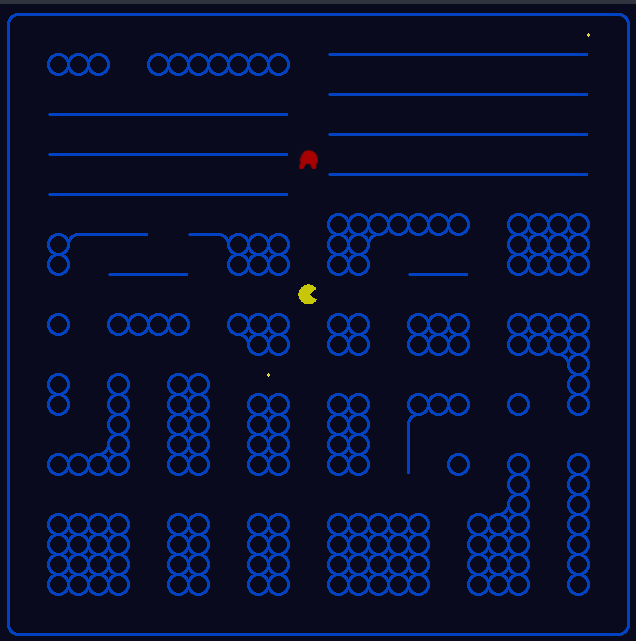
\includegraphics[width=350pt]{images/board_example}\\
					\caption{Example board. Walls, empty tiles, the player, coins and a red ghost are visible}
					\label{example_board}
				\end{img}
				General idea is that all border tiles of each level (tile system explained later) have to be walls, which creates a nice, outer border of the board with rounded edges.
			\subsection{Counters}
				Directly below the board, counters are located, these provide information on:
				\begin{enumerate}
					\item
						Number of coins eaten
					\item
						Number of coins that are required to be consumed before progressing to the next level
					\item
						Number of player lives
					\item
						Current level number
				\end{enumerate}
				\begin{img}
					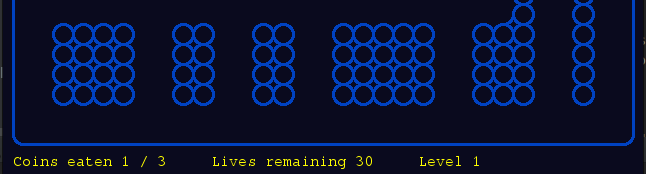
\includegraphics[width=350pt]{images/counter_example}\\
					\caption{Example set of counters with part of the board included for position reference.}
				\end{img}
				Every time the player eats a 'coin' the first counter increases. Throughout the level, this counter cannot decrease as even upon player's death, the already-eaten coins don't respawn.
				
				Number of coins required to progress is constant through the level but may differ between levels. It is worth mentioning that as every coin must be eaten to progress, this acts as a total number of coins allocated in each level map. Coin placing algorithm described later in this document also proves that it equals to $32^2-\#_{wall\_tiles}-\#_{empty\_ tiles}$.
				
				Each time a player comes in contact with a ghost(defined later in this document) a life is subtracted and every time the player eats a heart eatable, a life is added.
				
				Level number increases from 1 (easiest level) up to ten (hardest level), as player advances through the levels.
		\section{Grid layout}
			Pygame provides a sprite attribute of its location but as I have decided to use a window of over 500x500px of size, its pixel-accurate positioning would be an overkill and could make programming harder as well as require more processing power to (later mentioned) pathfinding algorithms.
			Due to this I have turned to the original PacMan solution (as read in Reference \ref{stronaopacmanie}), the grid system. The board was initially made as a 64x64 grid, where each piece, namely a tile, was either a wall or a space a sprite may move on. First levels were designed this way and I found the level design a really hard task. Only later I have noticed that the grid of the original PacMan was barely $\dfrac{1}{4}^{\text{th}}$ of the size I have used, my board was just to big for a pleasant gameplay.
			
			As I wanted the board to be square I have decided to move to 32x32 grid. Some testing later I have decided that this size not only nicely divides by 2 making perfectly symmetrical or even fractal levels possible to make but also is actually quite the one most similar in terms of number of tiles to the one the original PacMan had (for square boards).
			\begin{img}
				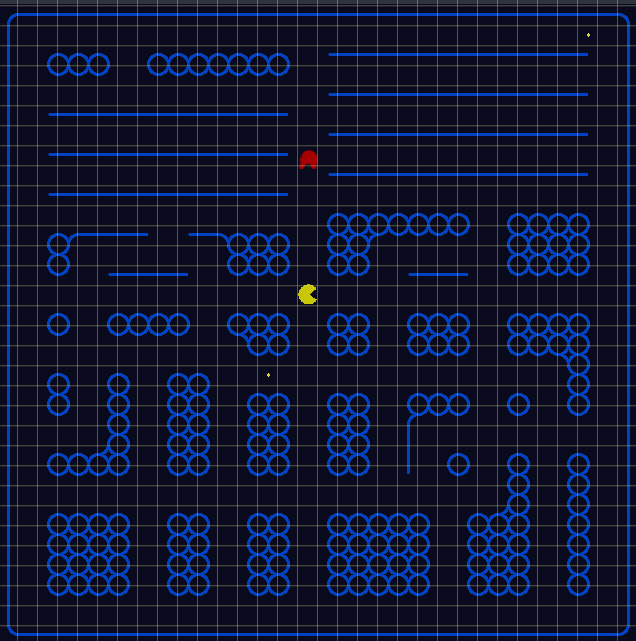
\includegraphics[width=350pt]{images/board_grid}\\
				\caption{Example of a board with a grid applied (note that the grid was added just for demonstrative purposes and in not a part of the game.)}
			\end{img}
			The following section describes types of different tiles used throughout the game.
		\section{Types of tiles}
			\subsection{Walls}
				
			\subsection{Player}
			\subsection{Ghosts}
			\subsection{Eatables}
				\subsubsection{Coins}
				\subsubsection{Hearts}
			\subsection{Empty tiles}
		\section{Levels}
			\subsection{Permanent storing}
			\subsection{Interpreting}
			\subsection{Storing while in game}
			\subsection{Designing the levels}
			\subsection{User-defined levels}
			\subsection{Progressing to the next level}
		\section{Gameplay scheme}
			\subsection{Player movement}
			\subsection{Ghost movement}
			\subsection{Eating}
			\subsection{Getting killed}
			\subsection{Respawning after a loss of life}
		\section{Types of message screens}
			\subsection{Tutorial}
			\subsection{Loss of life}
			\subsection{Completing the level}
			\subsection{Loosing the game}
			\subsection{Completing the entire game}
		\section{Testing}
	\chapter{References}
		\begin{enumerate}
			\item
				http://gameinternals.com/post/2072558330/understanding-pac-man-ghost-behavior
				\label{stronaopacmanie}
		\end{enumerate}
			
\end{document}